\documentclass[11pt
  , a4paper
  , article
  , oneside
  %  , twoside
  , showtrims
 % , draft
]{memoir}

\usepackage{essdocs}
\usepackage[numbers]{natbib}
\usepackage[autostyle]{csquotes}

\setsecnumdepth{subsection}

\begin{document}
%\frontmatter
%% ESS Document Description
%%
\essdocdesc{Engineering Manual}

%% ESS Document Number
%%
\essdocnum{ESS-0136437}

%% Date
%%
\date{\today}

%% ESS Document Revision Number
%%
\essdocrev{0.9}

%% ESS Document State
%%
\essdocstate{Draft}

%% ESS Document Classification
%%
\essdocclass{Public}

%% Document Title
%%
\title{ICS Engineering Manual}
\subtitle{for an Inventory System with JIRA and EPICS}
%% Document Author(s), if more than one author,
%% use \newline instead of \\ or \linebreak in order to seperate them
\author{Jeong Han Lee (han.lee@esss.se)}

%% Document Reviewer(s) if more than one reviewer,
%% use \newline instead of \\ or \linebreak in order to seperate them
%\reviewer{Timo Korhonen (Chief Engineer) \newline Timo Korhonen (Chief Engineer)}
\reviewer{TBD}
%% Document Owner(s) if more than one owner,
%% use \newline instead of \\ or \linebreak in order to seperate them
\owner{ICS}

%% Document Approver(s) if more than one approver,
%% use \newline instead of \\ or \linebreak in order to seperate them
\approver{ICS}

\showtrimson

\esstitle
\newpage
\tableofcontents
\newpage

%\mainmatter


%%% Actual Document Start at below
\chapter{Overview}
There are infinite ways to develop and maintain an inventory system. However, this inventory is the unique and \textbf{temporary} solution for the ICS Tuna Lab. This inventory system is designed to minimize resources when an engineer register bulky items to the existent JIRA ICS HW\&I group inventory task. Therefore, it does \textbf{NOT} provide any fancy and beautiful ways to interact with users, \textbf{BUT} does provide the minimal tool to monitor and track any equipment in ICS, ESS, and any IK partner. And the system only provide the following features :
\begin{itemize}
\item Do stock an item to JIRA, and do Add-and-Print its barcodes.
\item Do stock an item to JIRA, and do Add-and-Print its barcodes.
\item Delete an item from JIRA.
\item Print the existent (created) label (in case, the printer doesn't work properly)
\end{itemize}


\begin{figure}[!htb]
%  \centering
  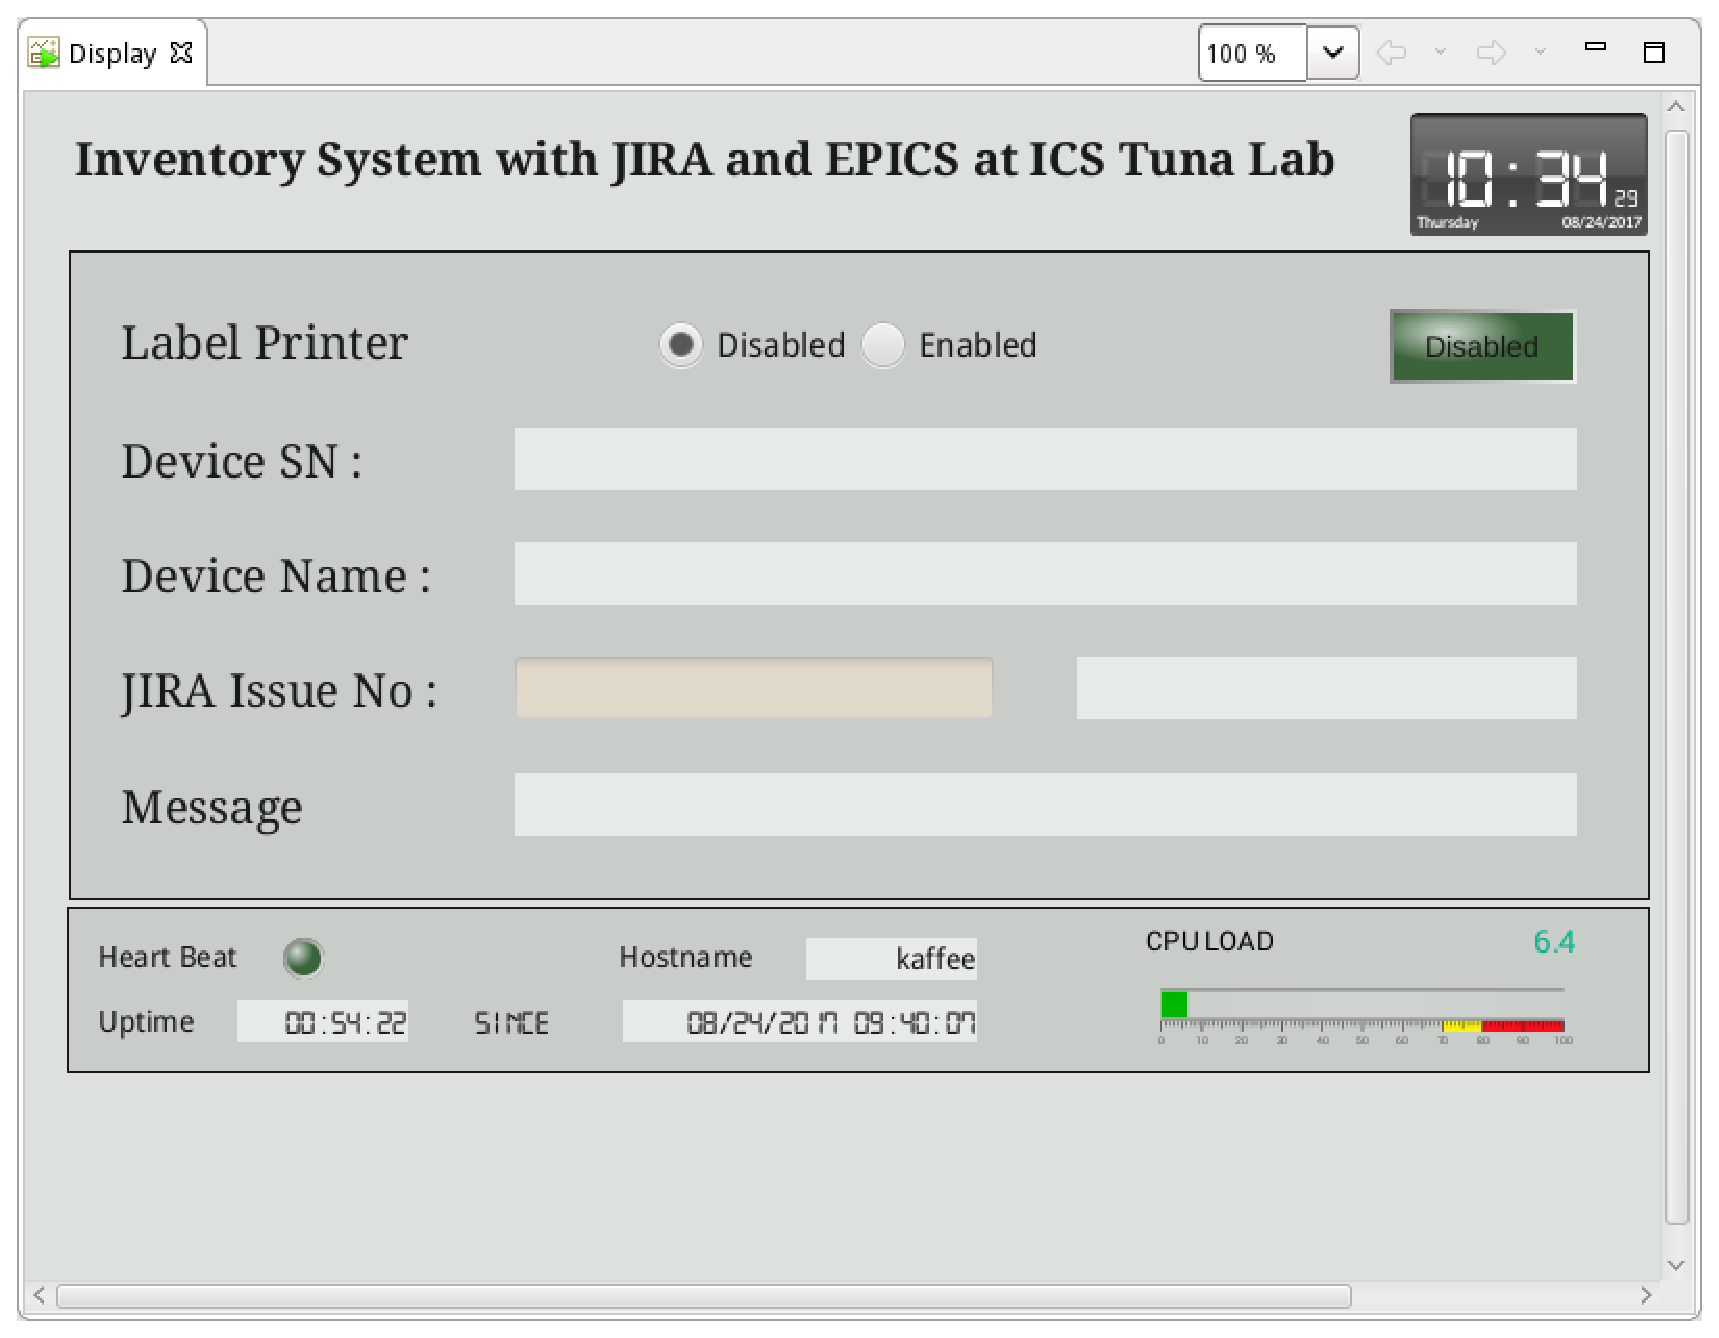
\includegraphics[width=0.5\textwidth]{./pictures/inv01.eps}
  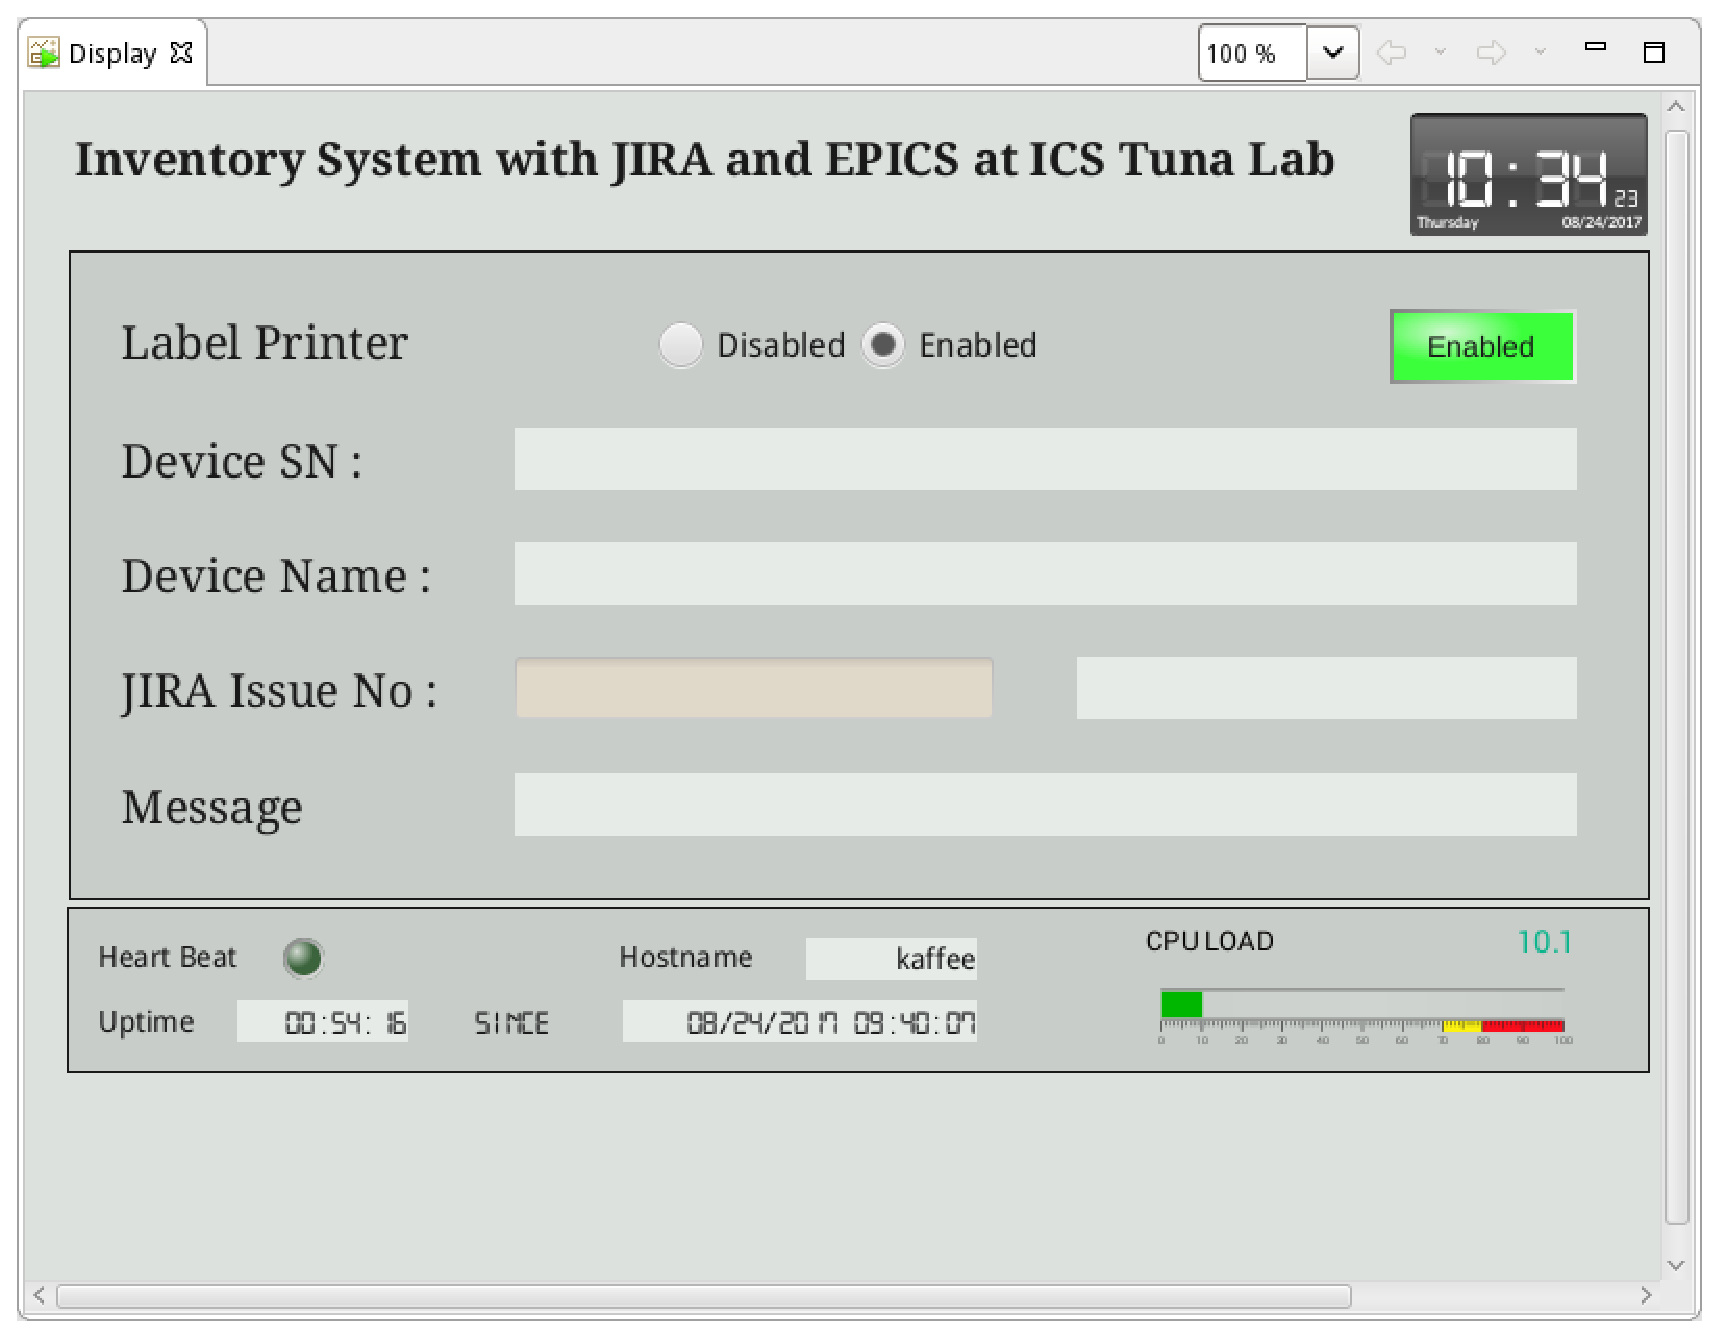
\includegraphics[width=0.5\textwidth]{./pictures/inv02.eps}
  \caption{
            CS-Studio User Interface Screen Examples.
          }
  \label{fig:css-examples}   
\end{figure}

\clearpage
\section{Inventory Workflow}

\subsection{How to stock an item at the first time to JIRA}

The mandatory steps are defined the following procedures :

\subsubsection{Scan the Serial Number on the equipment  with the Xenon 190x barcode scanner.}
\begin{figure}[!htb]
  \centering
  \includegraphics[width=0.35\textwidth,angle=90]{./pictures/01.eps}
  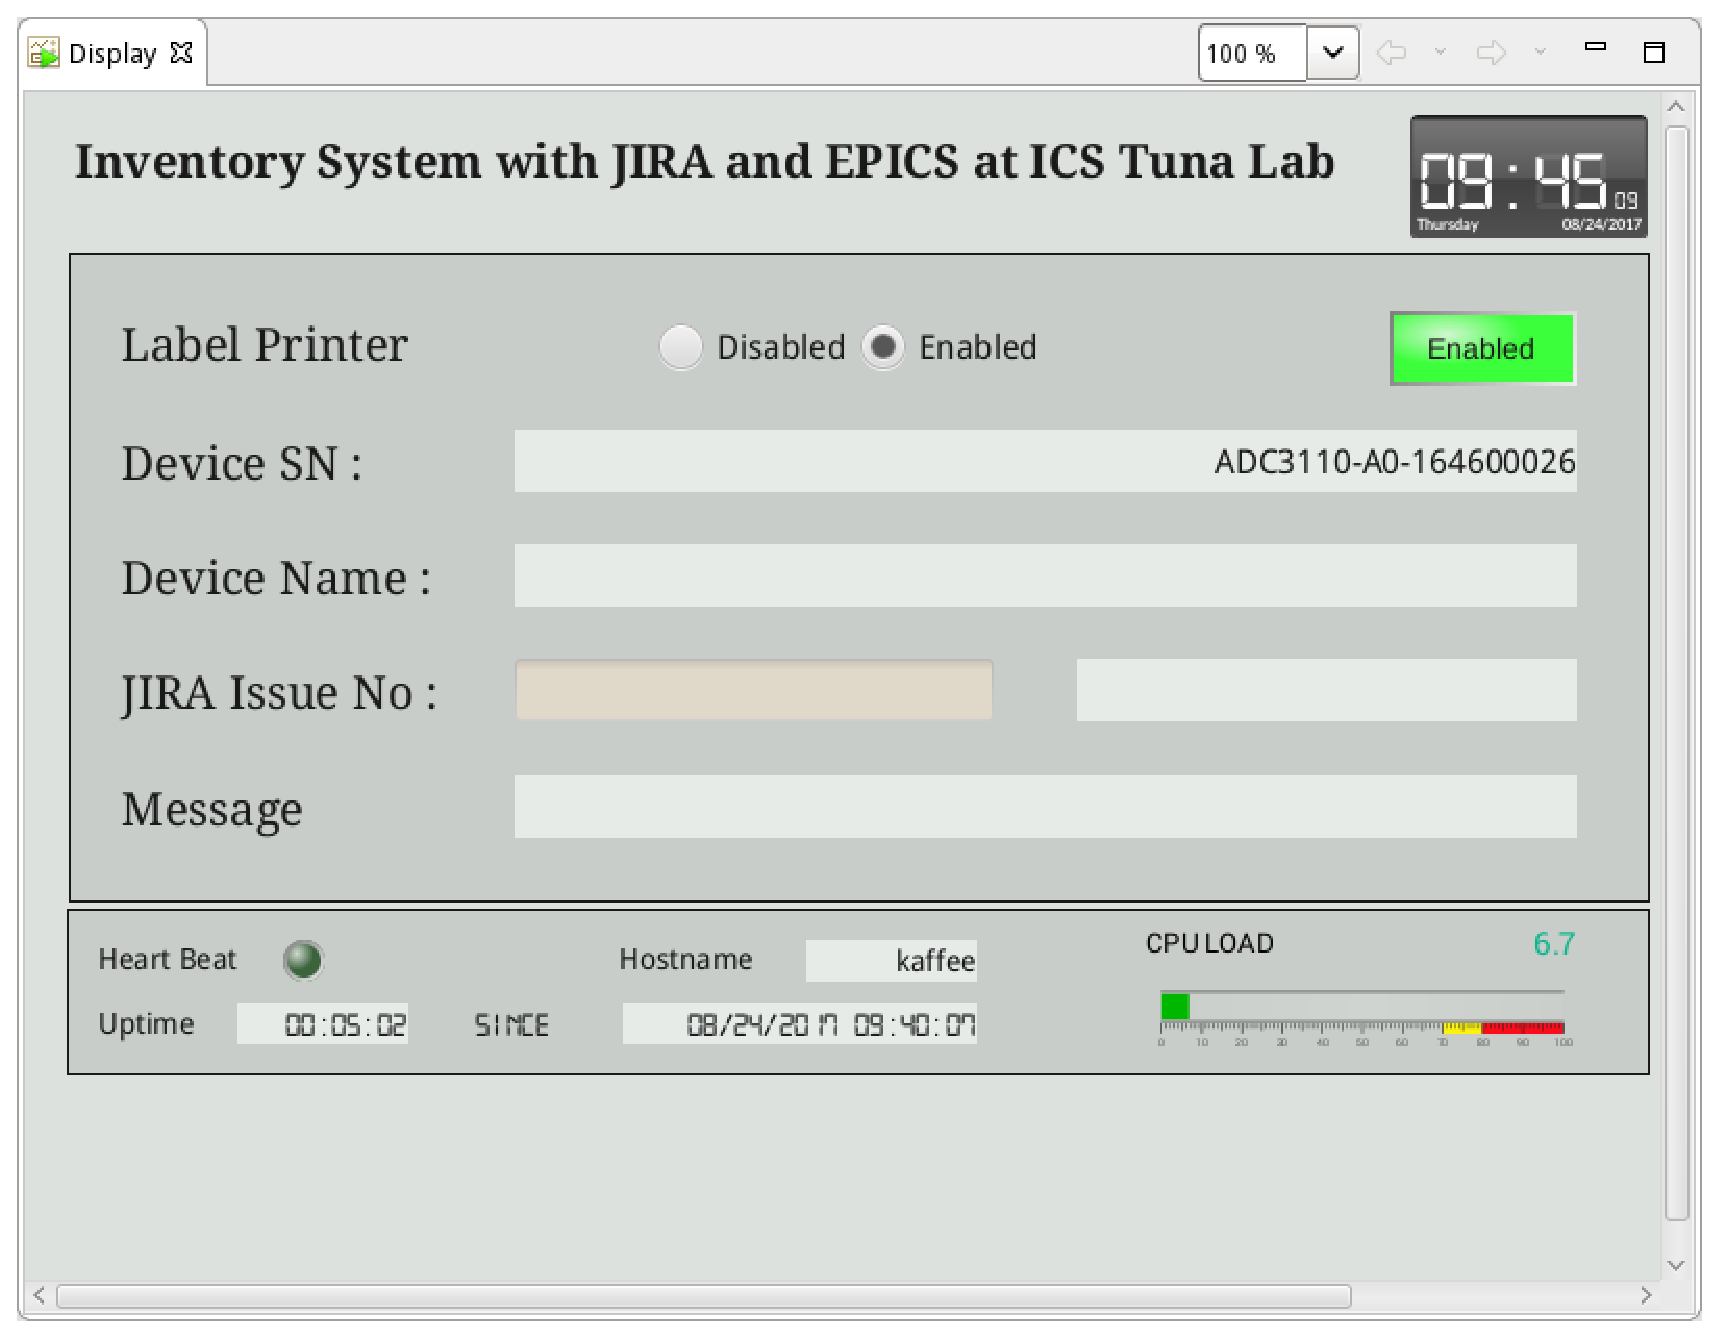
\includegraphics[width=0.45\textwidth]{./pictures/02.eps}
  \caption{
    User Interface Screen Example after the serial number scan. 
  }
\end{figure}

\subsubsection{Scan  one of 3.3 Model Codes in the manual with the Xenon 190x scanner.}
\begin{figure}[!htb]
  \centering
  \includegraphics[width=0.5\textwidth]{./pictures/03.eps}
  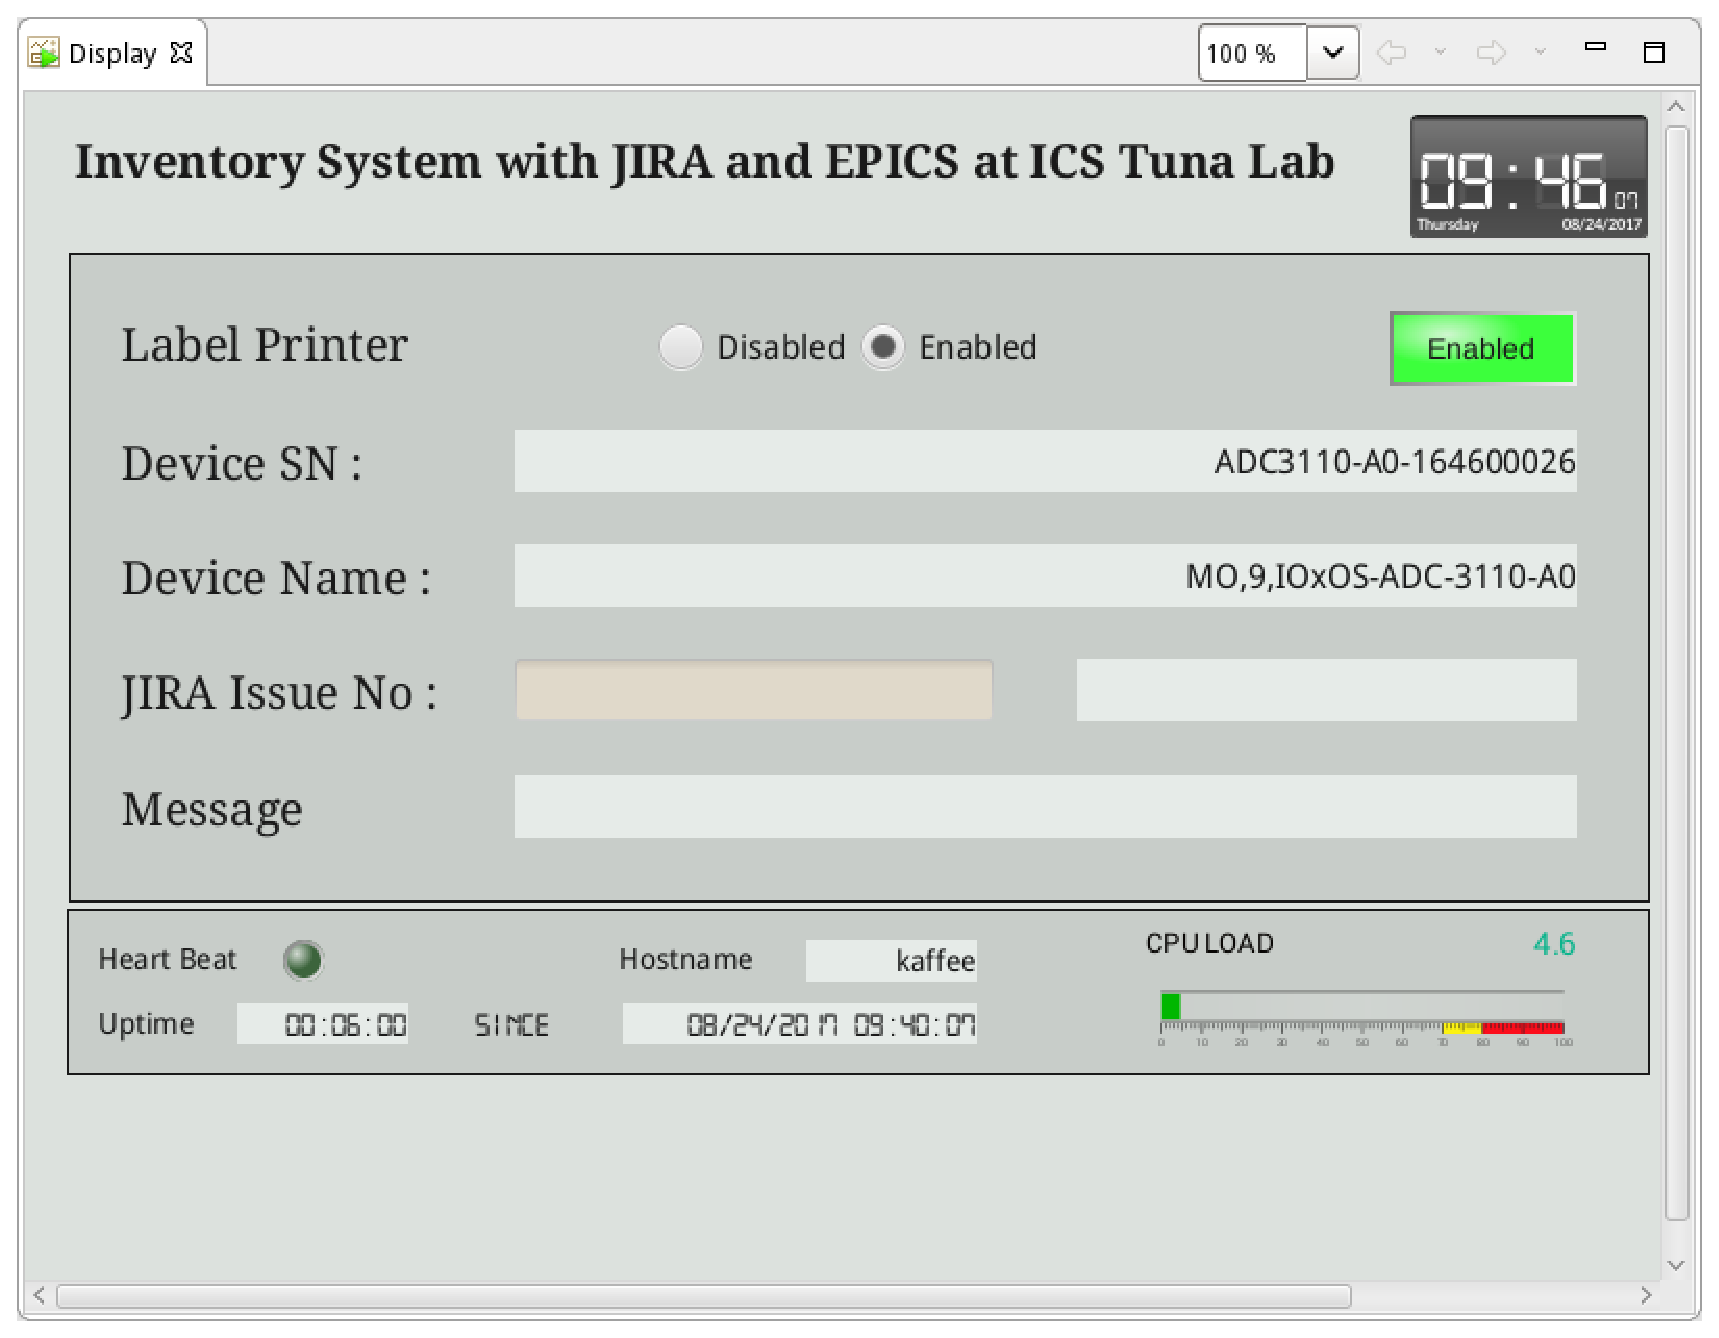
\includegraphics[width=0.484\textwidth]{./pictures/04.eps}
  \caption{
    User Interface Screen Example after the Model Name scan. 
  }
\end{figure}

\clearpage
\subsubsection{Both case in below, the created labels are attached in the JIRA issue.}

\begin{enumerate}
\item Scan Enable Label Printing after JIRA action if one wants to print labels (Default)
\item Scan Disable Label Printing after JIRA action if one wants not print labels
\end{enumerate}
\begin{figure}[!htb]
    \centering
    \includegraphics[width=0.36\textwidth,angle=90]{./pictures/05.eps}
    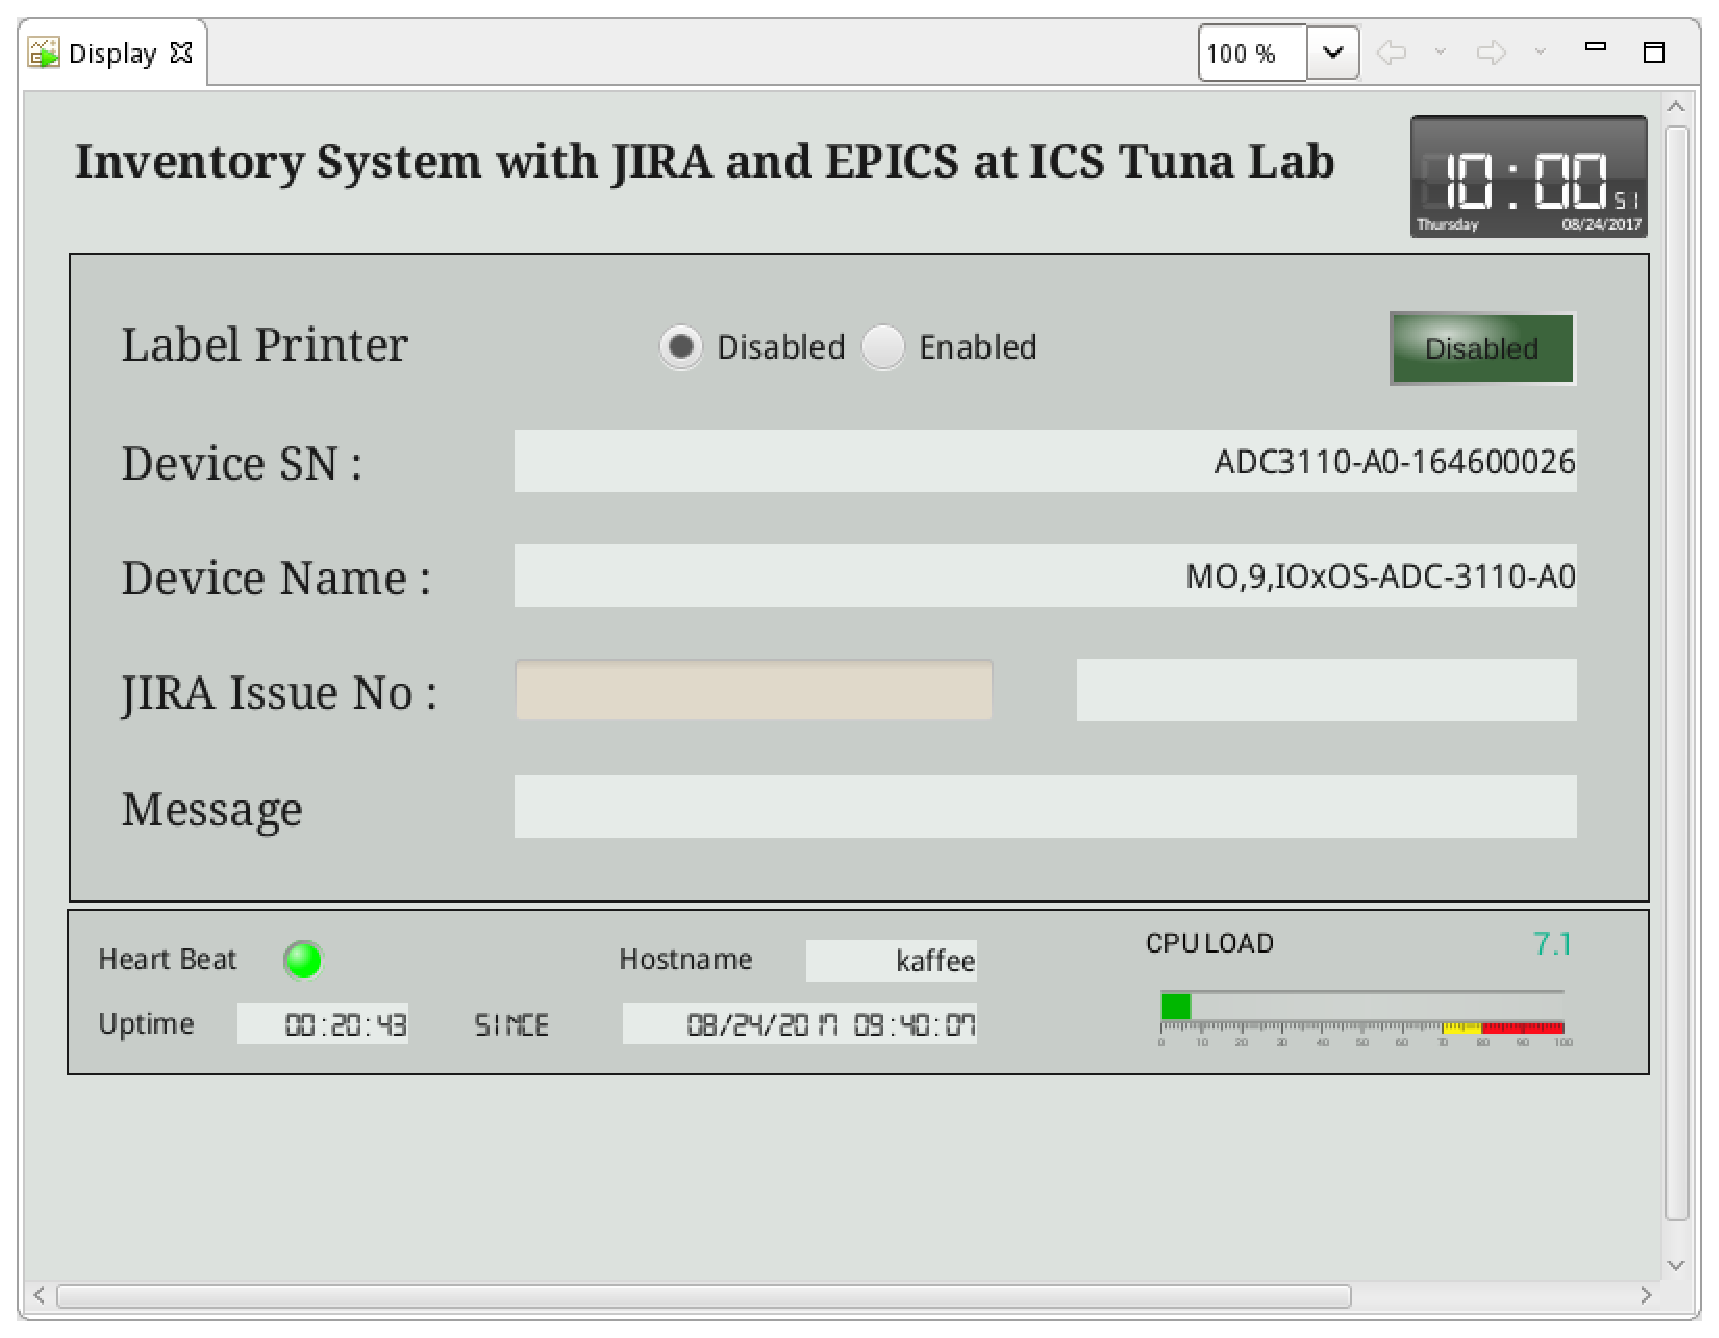
\includegraphics[width=0.466\textwidth]{./pictures/06.eps}
  \caption{
    User Interface Screen Example for Enable and Disable Labels
  }
\end{figure}

\subsubsection{Scan Create an JIRA issue in the manual}
\begin{figure}[!htb]
  \centering
  \includegraphics[width=0.5\textwidth]{./pictures/07.eps}
  \caption{
    User Interface Screen Example after the Create an JIRA scan. 
  }
\end{figure}

\clearpage
\subsubsection{Attach two barcodes in the reserved box, an equipment, or both.}
\begin{figure}[!htb]
    \centering
    \includegraphics[width=0.466\textwidth]{./pictures/09.eps}
    \includegraphics[width=0.466\textwidth]{./pictures/10.eps}
  \caption{
    Equipment with labels. The small one should be trimmed properly. 
  }
\end{figure}

\subsection{How to add and print barcodes for an Item which has registered in JIRA}

\begin{enumerate}
\item Define the TAG number which one wants to delete it via CS-Studio User Interface or caput \newline
  \texttt{caput ICSLAB:IssueNumber TAG-XXX}
\item Scan the Serial Number on the equipment  with the Xenon 190x barcode scanner.
\item Scan Model Name in the manual with the Xenon 190x scanner.
\item Both case in below, the updated labels are attached in the JIRA issue.
  \begin{enumerate}
  \item Scan Enable Label Printing after JIRA action if one wants to print the updated label (Default)
  \item Scan Disable Label Printing after JIRA action if one wants not print the updated label
  \end{enumerate}
\item Scan Update an JIRA issue in the engineering manual
\end{enumerate}


\subsection{How to delete the existent Item}

\begin{enumerate}
\item  Define the TAG number which one wants to delete it via  CS-Studio User Interface or caput \newline
\texttt{caput ICSLAB:IssueNumber TAG-XXX}
\item Scan Delete an JIRA issue Barcode in the manual with the Xenon 190x barcode scanner.
\end{enumerate}


\subsection{Print the existent labels}
In case, there is the printer issue, for example, print only one of two labels, not responding, and so on.
\begin{enumerate}
\item Please check the printer status at \url{http://localhost:631/} and resolve it. Note that one should know the basic CUPS configuration. 
\item Print the existent label by scanning the barcode (Print the last existent label) in the manual. Note that this action will print only the recent created labels. 
\end{enumerate}
\begin{figure}[!htb]
    \centering
    \includegraphics[width=0.4\textwidth,angle=90]{./pictures/11.eps}
    \caption{
    Bar code in the manual for the Print the Existent Label.
  }
\end{figure}

\clearpage
\section{Components}
\subsection{Hardware}
\begin{itemize}
\item Honeywell Xenon 1900g (Wire) or 1902g (Wireless) Barcode scanner
\item DYMO LabelWriter 450 Duo
\end{itemize}
\subsection{Software}
\begin{itemize}
\item Linux OS (tested with Debian 8) 
\item EPICS IOC  {\tiny \url{https://github.com/jeonghanlee/hw-xenon1900}}
\item JIRA {\tiny \url{https://jira.esss.lu.se/projects/TAG/summary}}
\item DYMO LabelWriter 450 Duo CUP Driver \newline
  {\tiny
  \url{http://www.dymo.com/en-US/dymo-label-sdk-and-cups-drivers-for-linux-dymo-label-sdk-cups-linux-p--1}}
\end{itemize}

\section{Troubleshooting}


\newpage
\chapter{Honeywell Xenon Scanners 1900 and 1902g}
Note that there are different procedure to setup Xenon 1900 corded scanner and Xenon 1902g cordless scanner. Please consult each manual in detail.


\section{Basic Configuration}
\begin{figure}[!htb]
%  \centering
  
\includegraphics[width=0.3\textwidth]{./pictures/scanner_settings_default.eps}
  \caption{
            Default Settings.
          }
  \label{fig:default}   
\end{figure}

\begin{figure}[!htb]
%  \centering
  
\includegraphics[width=0.3\textwidth]{./pictures/scanner_settings_usbserial.eps}
  \caption{
            USB Serial Setting.
          }
  \label{fig:usb-serial}   
\end{figure}


\begin{figure}[!htb]
%  \centering
  
\includegraphics[width=0.3\textwidth]{./pictures/scanner_settings_silent_corded.eps}
  \caption{
            Silent Mode for Corded Scanner.
          }
  \label{fig:silent-corded}   
\end{figure}



\begin{figure}[!htb]
%  \centering
  
\includegraphics[width=0.3\textwidth]{./pictures/scanner_settings_silent_cordless.eps}
  \caption{
            Silent Mode for Cordless Scanner.
          }
  \label{fig:silent-cordless}   
\end{figure}


% \chapter{Frequently Usage Case}
%% \section{MTCA}
%% \subsection{MTCA IOxOS IFC1410}
%% \subsection{MRF EVR-300DC}


%% \newpage
%% \section{Network Device}
%% \subsection{MOXA Nport 6650}
%% \subsection{HP Network Switch}

\newpage
\chapter{Predefined Bar Codes}
%% \section{Vendor Codes}
%% \vspace{1cm}
%% \noindent
\vspace{1.4cm}
\begin{minipage}{.2\textwidth}
\begin{center}

\includegraphics[height=1cm,keepaspectratio]{/home/jhlee/gitsrc/hw-xenon1900/docs/zint/vd_images/undefined.eps}
\end{center}
\end{minipage}
\begin{minipage}{.7\textwidth}
undefined
\end{minipage}


\noindent
\vspace{1.4cm}
\begin{minipage}{.2\textwidth}
\begin{center}

\includegraphics[height=1cm,keepaspectratio]{/home/jhlee/gitsrc/hw-xenon1900/docs/zint/vd_images/ess.eps}
\end{center}
\end{minipage}
\begin{minipage}{.7\textwidth}
ess
\end{minipage}


\noindent
\vspace{1.4cm}
\begin{minipage}{.2\textwidth}
\begin{center}

\includegraphics[height=1cm,keepaspectratio]{/home/jhlee/gitsrc/hw-xenon1900/docs/zint/vd_images/mrf.eps}
\end{center}
\end{minipage}
\begin{minipage}{.7\textwidth}
mrf
\end{minipage}


\noindent
\vspace{1.4cm}
\begin{minipage}{.2\textwidth}
\begin{center}

\includegraphics[height=1cm,keepaspectratio]{/home/jhlee/gitsrc/hw-xenon1900/docs/zint/vd_images/ioxos.eps}
\end{center}
\end{minipage}
\begin{minipage}{.7\textwidth}
ioxos
\end{minipage}


\noindent
\vspace{1.4cm}
\begin{minipage}{.2\textwidth}
\begin{center}

\includegraphics[height=1cm,keepaspectratio]{/home/jhlee/gitsrc/hw-xenon1900/docs/zint/vd_images/wiener.eps}
\end{center}
\end{minipage}
\begin{minipage}{.7\textwidth}
wiener
\end{minipage}


\noindent
\vspace{1.4cm}
\begin{minipage}{.2\textwidth}
\begin{center}

\includegraphics[height=1cm,keepaspectratio]{/home/jhlee/gitsrc/hw-xenon1900/docs/zint/vd_images/moxa.eps}
\end{center}
\end{minipage}
\begin{minipage}{.7\textwidth}
moxa
\end{minipage}


\noindent
\vspace{1.4cm}
\begin{minipage}{.2\textwidth}
\begin{center}

\includegraphics[height=1cm,keepaspectratio]{/home/jhlee/gitsrc/hw-xenon1900/docs/zint/vd_images/nat.eps}
\end{center}
\end{minipage}
\begin{minipage}{.7\textwidth}
nat
\end{minipage}


\noindent
\vspace{1.4cm}
\begin{minipage}{.2\textwidth}
\begin{center}

\includegraphics[height=1cm,keepaspectratio]{/home/jhlee/gitsrc/hw-xenon1900/docs/zint/vd_images/concurrent.eps}
\end{center}
\end{minipage}
\begin{minipage}{.7\textwidth}
concurrent
\end{minipage}


\noindent
\vspace{1.4cm}
\begin{minipage}{.2\textwidth}
\begin{center}

\includegraphics[height=1cm,keepaspectratio]{/home/jhlee/gitsrc/hw-xenon1900/docs/zint/vd_images/schroff.eps}
\end{center}
\end{minipage}
\begin{minipage}{.7\textwidth}
schroff
\end{minipage}


\noindent
\vspace{1.4cm}
\begin{minipage}{.2\textwidth}
\begin{center}

\includegraphics[height=1cm,keepaspectratio]{/home/jhlee/gitsrc/hw-xenon1900/docs/zint/vd_images/struck.eps}
\end{center}
\end{minipage}
\begin{minipage}{.7\textwidth}
struck
\end{minipage}


\noindent
\vspace{1.4cm}
\begin{minipage}{.2\textwidth}
\begin{center}

\includegraphics[height=1cm,keepaspectratio]{/home/jhlee/gitsrc/hw-xenon1900/docs/zint/vd_images/dell.eps}
\end{center}
\end{minipage}
\begin{minipage}{.7\textwidth}
dell
\end{minipage}


\noindent
\vspace{1.4cm}
\begin{minipage}{.2\textwidth}
\begin{center}

\includegraphics[height=1cm,keepaspectratio]{/home/jhlee/gitsrc/hw-xenon1900/docs/zint/vd_images/samsung.eps}
\end{center}
\end{minipage}
\begin{minipage}{.7\textwidth}
samsung
\end{minipage}


\noindent
\vspace{1.4cm}
\begin{minipage}{.2\textwidth}
\begin{center}

\includegraphics[height=1cm,keepaspectratio]{/home/jhlee/gitsrc/hw-xenon1900/docs/zint/vd_images/hp.eps}
\end{center}
\end{minipage}
\begin{minipage}{.7\textwidth}
hp
\end{minipage}


\noindent
\vspace{1.4cm}
\begin{minipage}{.2\textwidth}
\begin{center}

\includegraphics[height=1cm,keepaspectratio]{/home/jhlee/gitsrc/hw-xenon1900/docs/zint/vd_images/ibm.eps}
\end{center}
\end{minipage}
\begin{minipage}{.7\textwidth}
ibm
\end{minipage}


\noindent
\vspace{1.4cm}
\begin{minipage}{.2\textwidth}
\begin{center}

\includegraphics[height=1cm,keepaspectratio]{/home/jhlee/gitsrc/hw-xenon1900/docs/zint/vd_images/caen.eps}
\end{center}
\end{minipage}
\begin{minipage}{.7\textwidth}
caen
\end{minipage}


\noindent
\vspace{1.4cm}
\begin{minipage}{.2\textwidth}
\begin{center}

\includegraphics[height=1cm,keepaspectratio]{/home/jhlee/gitsrc/hw-xenon1900/docs/zint/vd_images/raritan.eps}
\end{center}
\end{minipage}
\begin{minipage}{.7\textwidth}
raritan
\end{minipage}


\noindent
\vspace{1.4cm}
\begin{minipage}{.2\textwidth}
\begin{center}

\includegraphics[height=1cm,keepaspectratio]{/home/jhlee/gitsrc/hw-xenon1900/docs/zint/vd_images/dymo.eps}
\end{center}
\end{minipage}
\begin{minipage}{.7\textwidth}
dymo
\end{minipage}




%% \newpage
%% \section{FormFactor Codes}
%% \vspace{1cm}
%% \noindent
\vspace{1.4cm}
\begin{minipage}{.2\textwidth}
\begin{center}

\includegraphics[height=1cm,keepaspectratio]{/home/jhlee/epics_env/epics-Apps/hw-xenon1900/docs/zint/ff_images/undefined.eps}
\end{center}
\end{minipage}
\begin{minipage}{.7\textwidth}
undefined
\end{minipage}


\noindent
\vspace{1.4cm}
\begin{minipage}{.2\textwidth}
\begin{center}

\includegraphics[height=1cm,keepaspectratio]{/home/jhlee/epics_env/epics-Apps/hw-xenon1900/docs/zint/ff_images/mtca.eps}
\end{center}
\end{minipage}
\begin{minipage}{.7\textwidth}
mtca
\end{minipage}


\noindent
\vspace{1.4cm}
\begin{minipage}{.2\textwidth}
\begin{center}

\includegraphics[height=1cm,keepaspectratio]{/home/jhlee/epics_env/epics-Apps/hw-xenon1900/docs/zint/ff_images/pcie.eps}
\end{center}
\end{minipage}
\begin{minipage}{.7\textwidth}
pcie
\end{minipage}


\noindent
\vspace{1.4cm}
\begin{minipage}{.2\textwidth}
\begin{center}

\includegraphics[height=1cm,keepaspectratio]{/home/jhlee/epics_env/epics-Apps/hw-xenon1900/docs/zint/ff_images/cpci.eps}
\end{center}
\end{minipage}
\begin{minipage}{.7\textwidth}
cpci
\end{minipage}


\noindent
\vspace{1.4cm}
\begin{minipage}{.2\textwidth}
\begin{center}

\includegraphics[height=1cm,keepaspectratio]{/home/jhlee/epics_env/epics-Apps/hw-xenon1900/docs/zint/ff_images/pmc.eps}
\end{center}
\end{minipage}
\begin{minipage}{.7\textwidth}
pmc
\end{minipage}


\noindent
\vspace{1.4cm}
\begin{minipage}{.2\textwidth}
\begin{center}

\includegraphics[height=1cm,keepaspectratio]{/home/jhlee/epics_env/epics-Apps/hw-xenon1900/docs/zint/ff_images/vme.eps}
\end{center}
\end{minipage}
\begin{minipage}{.7\textwidth}
vme
\end{minipage}




%% \newpage
%% \section{ICS Location Codes}
%% \vspace{1cm}
%% \noindent
\vspace{1.4cm}
\begin{minipage}{.2\textwidth}
\begin{center}

\includegraphics[height=1cm,keepaspectratio]{/home/jhlee/epics_env/epics-Apps/hw-xenon1900/docs/zint/lo_images/undefined.eps}
\end{center}
\end{minipage}
\begin{minipage}{.7\textwidth}
undefined
\end{minipage}




%% \newpage
%% \section{Status Codes}
%% \vspace{1cm}
%% \noindent
\vspace{1.4cm}
\begin{minipage}{.2\textwidth}
\begin{center}

\includegraphics[height=1cm,keepaspectratio]{/home/jhlee/epics_env/epics-Apps/hw-xenon1900/manual/zint/st_images/undefined.eps}
\end{center}
\end{minipage}
\begin{minipage}{.7\textwidth}
undefined
\end{minipage}


\noindent
\vspace{1.4cm}
\begin{minipage}{.2\textwidth}
\begin{center}

\includegraphics[height=1cm,keepaspectratio]{/home/jhlee/epics_env/epics-Apps/hw-xenon1900/manual/zint/st_images/stock.eps}
\end{center}
\end{minipage}
\begin{minipage}{.7\textwidth}
stock
\end{minipage}


\noindent
\vspace{1.4cm}
\begin{minipage}{.2\textwidth}
\begin{center}

\includegraphics[height=1cm,keepaspectratio]{/home/jhlee/epics_env/epics-Apps/hw-xenon1900/manual/zint/st_images/inservice.eps}
\end{center}
\end{minipage}
\begin{minipage}{.7\textwidth}
inservice
\end{minipage}


\noindent
\vspace{1.4cm}
\begin{minipage}{.2\textwidth}
\begin{center}

\includegraphics[height=1cm,keepaspectratio]{/home/jhlee/epics_env/epics-Apps/hw-xenon1900/manual/zint/st_images/disposed.eps}
\end{center}
\end{minipage}
\begin{minipage}{.7\textwidth}
disposed
\end{minipage}




\section{Model Codes}
\vspace{1cm}
\noindent
\vspace{1cm}
\begin{minipage}{.2\textwidth}
\begin{center}

\includegraphics[height=1cm,keepaspectratio]{/home/jhlee/gitsrc/hw-xenon1900/manual/zint/mo_images/undefined.eps}
\end{center}
\end{minipage}
\begin{minipage}{.7\textwidth}
UNDEFINED
\end{minipage}


\noindent
\vspace{1cm}
\begin{minipage}{.2\textwidth}
\begin{center}

\includegraphics[height=1cm,keepaspectratio]{/home/jhlee/gitsrc/hw-xenon1900/manual/zint/mo_images/mtca-evm-300.eps}
\end{center}
\end{minipage}
\begin{minipage}{.7\textwidth}
MTCA-EVM-300
\end{minipage}


\noindent
\vspace{1cm}
\begin{minipage}{.2\textwidth}
\begin{center}

\includegraphics[height=1cm,keepaspectratio]{/home/jhlee/gitsrc/hw-xenon1900/manual/zint/mo_images/vme-evm-300.eps}
\end{center}
\end{minipage}
\begin{minipage}{.7\textwidth}
VME-EVM-300
\end{minipage}


\noindent
\vspace{1cm}
\begin{minipage}{.2\textwidth}
\begin{center}

\includegraphics[height=1cm,keepaspectratio]{/home/jhlee/gitsrc/hw-xenon1900/manual/zint/mo_images/pcie-evr-300.eps}
\end{center}
\end{minipage}
\begin{minipage}{.7\textwidth}
PCIE-EVR-300
\end{minipage}


\noindent
\vspace{1cm}
\begin{minipage}{.2\textwidth}
\begin{center}

\includegraphics[height=1cm,keepaspectratio]{/home/jhlee/gitsrc/hw-xenon1900/manual/zint/mo_images/pcie-evr-300dc.eps}
\end{center}
\end{minipage}
\begin{minipage}{.7\textwidth}
PCIE-EVR-300DC
\end{minipage}


\noindent
\vspace{1cm}
\begin{minipage}{.2\textwidth}
\begin{center}

\includegraphics[height=1cm,keepaspectratio]{/home/jhlee/gitsrc/hw-xenon1900/manual/zint/mo_images/pmc-evr-230.eps}
\end{center}
\end{minipage}
\begin{minipage}{.7\textwidth}
PMC-EVR-230
\end{minipage}


\noindent
\vspace{1cm}
\begin{minipage}{.2\textwidth}
\begin{center}
\includegraphics[height=1cm,keepaspectratio]{/home/jhlee/gitsrc/hw-xenon1900/manual/zint/mo_images/vme-evr-230.eps}
\end{center}
\end{minipage}
\begin{minipage}{.7\textwidth}
VME-EVR-230
\end{minipage}


\noindent
\vspace{1cm}
\begin{minipage}{.2\textwidth}
\begin{center}
\includegraphics[height=1cm,keepaspectratio]{/home/jhlee/gitsrc/hw-xenon1900/manual/zint/mo_images/vme-evr-230rf.eps}
\end{center}
\end{minipage}
\begin{minipage}{.7\textwidth}
VME-EVR-230RF
\end{minipage}


\noindent
\vspace{1cm}
\begin{minipage}{.2\textwidth}
\begin{center}
\includegraphics[height=1cm,keepaspectratio]{/home/jhlee/gitsrc/hw-xenon1900/manual/zint/mo_images/cpci-evr-230.eps}
\end{center}
\end{minipage}
\begin{minipage}{.7\textwidth}
CPCI-EVR-230
\end{minipage}


\noindent
\vspace{1cm}
\begin{minipage}{.2\textwidth}
\begin{center}
\includegraphics[height=1cm,keepaspectratio]{/home/jhlee/gitsrc/hw-xenon1900/manual/zint/mo_images/vme-fout-12.eps}
\end{center}
\end{minipage}
\begin{minipage}{.7\textwidth}
VME-FOUT-12
\end{minipage}


\noindent
\vspace{1cm}
\begin{minipage}{.2\textwidth}
\begin{center}
\includegraphics[height=1cm,keepaspectratio]{/home/jhlee/gitsrc/hw-xenon1900/manual/zint/mo_images/cpci-fout-12.eps}
\end{center}
\end{minipage}
\begin{minipage}{.7\textwidth}
CPCI-FOUT-12
\end{minipage}


\noindent
\vspace{1cm}
\begin{minipage}{.2\textwidth}
\begin{center}
\includegraphics[height=1cm,keepaspectratio]{/home/jhlee/gitsrc/hw-xenon1900/manual/zint/mo_images/cpci-evg-220.eps}
\end{center}
\end{minipage}
\begin{minipage}{.7\textwidth}
CPCI-EVG-220
\end{minipage}


\noindent
\vspace{1cm}
\begin{minipage}{.2\textwidth}
\begin{center}
\includegraphics[height=1cm,keepaspectratio]{/home/jhlee/gitsrc/hw-xenon1900/manual/zint/mo_images/cpci-evg-230.eps}
\end{center}
\end{minipage}
\begin{minipage}{.7\textwidth}
CPCI-EVG-230
\end{minipage}


\noindent
\vspace{1cm}
\begin{minipage}{.2\textwidth}
\begin{center}
\includegraphics[height=1cm,keepaspectratio]{/home/jhlee/gitsrc/hw-xenon1900/manual/zint/mo_images/vme-evg-230.eps}
\end{center}
\end{minipage}
\begin{minipage}{.7\textwidth}
VME-EVG-230
\end{minipage}


\noindent
\vspace{1cm}
\begin{minipage}{.2\textwidth}
\begin{center}
\includegraphics[height=1cm,keepaspectratio]{/home/jhlee/gitsrc/hw-xenon1900/manual/zint/mo_images/nport5510.eps}
\end{center}
\end{minipage}
\begin{minipage}{.7\textwidth}
NPORT5510
\end{minipage}


\noindent
\vspace{1cm}
\begin{minipage}{.2\textwidth}
\begin{center}
\includegraphics[height=1cm,keepaspectratio]{/home/jhlee/gitsrc/hw-xenon1900/manual/zint/mo_images/nport6650.eps}
\end{center}
\end{minipage}
\begin{minipage}{.7\textwidth}
NPORT6650
\end{minipage}


\noindent
\vspace{1cm}
\begin{minipage}{.2\textwidth}
\begin{center}
\includegraphics[height=1cm,keepaspectratio]{/home/jhlee/gitsrc/hw-xenon1900/manual/zint/mo_images/wienercrate450.eps}
\end{center}
\end{minipage}
\begin{minipage}{.7\textwidth}
WIENERCRATE450
\end{minipage}


\noindent
\vspace{1cm}
\begin{minipage}{.2\textwidth}
\begin{center}
\includegraphics[height=1cm,keepaspectratio]{/home/jhlee/gitsrc/hw-xenon1900/manual/zint/mo_images/pdu-x3-3600.eps}
\end{center}
\end{minipage}
\begin{minipage}{.7\textwidth}
PDU-X3-3600
\end{minipage}





\newpage
\chapter{Action Bar Codes}
\vspace{1cm}
\noindent
\vspace{1.4cm}
\begin{minipage}{.2\textwidth}
\begin{center}
\includegraphics[height=1cm,keepaspectratio]{/home/jhlee/gitsrc/hw-xenon1900/docs/zint/act_images/CL.eps}
\end{center}
\end{minipage}
\begin{minipage}{.7\textwidth}
Clear all scanned PVs
\end{minipage}


\noindent
\vspace{1.4cm}
\begin{minipage}{.2\textwidth}
\begin{center}
\includegraphics[height=1cm,keepaspectratio]{/home/jhlee/gitsrc/hw-xenon1900/docs/zint/act_images/00.eps}
\end{center}
\end{minipage}
\begin{minipage}{.7\textwidth}
----------- place holder ----------
\end{minipage}


\noindent
\vspace{1.4cm}
\begin{minipage}{.2\textwidth}
\begin{center}
\includegraphics[height=1cm,keepaspectratio]{/home/jhlee/gitsrc/hw-xenon1900/docs/zint/act_images/LE.eps}
\end{center}
\end{minipage}
\begin{minipage}{.7\textwidth}
Enable Label Printing after JIRA action (JC)
\end{minipage}


\noindent
\vspace{1.4cm}
\begin{minipage}{.2\textwidth}
\begin{center}
\includegraphics[height=1cm,keepaspectratio]{/home/jhlee/gitsrc/hw-xenon1900/docs/zint/act_images/LD.eps}
\end{center}
\end{minipage}
\begin{minipage}{.7\textwidth}
Disable Label Printing after JIRA action (JC)
\end{minipage}


\noindent
\vspace{1.4cm}
\begin{minipage}{.2\textwidth}
\begin{center}
\includegraphics[height=1cm,keepaspectratio]{/home/jhlee/gitsrc/hw-xenon1900/docs/zint/act_images/00.eps}
\end{center}
\end{minipage}
\begin{minipage}{.7\textwidth}
----------- place holder ----------
\end{minipage}


\noindent
\vspace{1.4cm}
\begin{minipage}{.2\textwidth}
\begin{center}
\includegraphics[height=1cm,keepaspectratio]{/home/jhlee/gitsrc/hw-xenon1900/docs/zint/act_images/JC.eps}
\end{center}
\end{minipage}
\begin{minipage}{.7\textwidth}
Create an JIRA issue 
\end{minipage}


\noindent
\vspace{1.4cm}
\begin{minipage}{.2\textwidth}
\begin{center}
\includegraphics[height=1cm,keepaspectratio]{/home/jhlee/gitsrc/hw-xenon1900/docs/zint/act_images/JU.eps}
\end{center}
\end{minipage}
\begin{minipage}{.7\textwidth}
Update an JIRA issue (Scan Hash ID and other fields first)
\end{minipage}


\noindent
\vspace{1.4cm}
\begin{minipage}{.2\textwidth}
\begin{center}
\includegraphics[height=1cm,keepaspectratio]{/home/jhlee/gitsrc/hw-xenon1900/docs/zint/act_images/JD.eps}
\end{center}
\end{minipage}
\begin{minipage}{.7\textwidth}
Delete an JIRA issue (Scan Hash ID first)
\end{minipage}


\noindent
\vspace{1.4cm}
\begin{minipage}{.2\textwidth}
\begin{center}
\includegraphics[height=1cm,keepaspectratio]{/home/jhlee/gitsrc/hw-xenon1900/docs/zint/act_images/JI.eps}
\end{center}
\end{minipage}
\begin{minipage}{.7\textwidth}
Define the Child (Scan Hash ID later)
\end{minipage}


\noindent
\vspace{1.4cm}
\begin{minipage}{.2\textwidth}
\begin{center}
\includegraphics[height=1cm,keepaspectratio]{/home/jhlee/gitsrc/hw-xenon1900/docs/zint/act_images/JP.eps}
\end{center}
\end{minipage}
\begin{minipage}{.7\textwidth}
Define the Parent (Scan Hash ID later)
\end{minipage}


\noindent
\vspace{1.4cm}
\begin{minipage}{.2\textwidth}
\begin{center}
\includegraphics[height=1cm,keepaspectratio]{/home/jhlee/gitsrc/hw-xenon1900/docs/zint/act_images/00.eps}
\end{center}
\end{minipage}
\begin{minipage}{.7\textwidth}
----------- place holder ----------
\end{minipage}


\noindent
\vspace{1.4cm}
\begin{minipage}{.2\textwidth}
\begin{center}
\includegraphics[height=1cm,keepaspectratio]{/home/jhlee/gitsrc/hw-xenon1900/docs/zint/act_images/PJ.eps}
\end{center}
\end{minipage}
\begin{minipage}{.7\textwidth}
Save and append each scanned PV to CSV file which JIRA can import  (per day)
\end{minipage}


\noindent
\vspace{1.4cm}
\begin{minipage}{.2\textwidth}
\begin{center}
\includegraphics[height=1cm,keepaspectratio]{/home/jhlee/gitsrc/hw-xenon1900/docs/zint/act_images/DJ.eps}
\end{center}
\end{minipage}
\begin{minipage}{.7\textwidth}
Push the scanned PVs to RDB and JIRA
\end{minipage}


\noindent
\vspace{1.4cm}
\begin{minipage}{.2\textwidth}
\begin{center}
\includegraphics[height=1cm,keepaspectratio]{/home/jhlee/gitsrc/hw-xenon1900/docs/zint/act_images/PD.eps}
\end{center}
\end{minipage}
\begin{minipage}{.7\textwidth}
Push the scanned PVs to RDB
\end{minipage}


\noindent
\vspace{1.4cm}
\begin{minipage}{.2\textwidth}
\begin{center}
\includegraphics[height=1cm,keepaspectratio]{/home/jhlee/gitsrc/hw-xenon1900/docs/zint/act_images/00.eps}
\end{center}
\end{minipage}
\begin{minipage}{.7\textwidth}
----------- place holder ----------
\end{minipage}


\noindent
\vspace{1.4cm}
\begin{minipage}{.2\textwidth}
\begin{center}
\includegraphics[height=1cm,keepaspectratio]{/home/jhlee/gitsrc/hw-xenon1900/docs/zint/act_images/SV.eps}
\end{center}
\end{minipage}
\begin{minipage}{.7\textwidth}
Save and overwrite each scanned PV in each csv file (per second)
\end{minipage}


\noindent
\vspace{1.4cm}
\begin{minipage}{.2\textwidth}
\begin{center}
\includegraphics[height=1cm,keepaspectratio]{/home/jhlee/gitsrc/hw-xenon1900/docs/zint/act_images/SJ.eps}
\end{center}
\end{minipage}
\begin{minipage}{.7\textwidth}
Save and overwrite each scanned PV in each json file (per second)
\end{minipage}





\chapter{Summary}

The system has the limited functionality for the usage of ICS Tuna Lab, since ICS would like to save at least 5 mins while stocking an equipment into the existent JIRA project. The system fulfilled the early and limited requirement, i.e., saving 5 mins per an equipment. Therefore, this development was ended. The system is now running in the ICS Lab. 

However, it may be the good starting point if one wants to implement the system with any relational database, which is more flexible than the restricted JIRA project, which cannot be modified with the current permission.

If one has any questions and comments on this system, please contact the developer through \href{mailto:han.lee@esss.se}{han.lee@esss.se}.

\end{document}
